% 10,11 and 12pt fonts allowed
\documentclass[12pt]{novax} 

% extend the number of registers
\usepackage{etex} 

\usepackage[margin={1.2in}]{geometry}
% \usepackage[top=1in,left=1in,vmarginratio=2:3,hmarginratio=2:5,twoside]{geometry}

% Appendix package. Not necessary, but it does make managing appendices easier
\usepackage[titletoc]{appendix}

% sideways tables and figures
\usepackage{rotating}

% tables that spill over multiple pages
\usepackage{longtable}

% references
\usepackage[square,sort,comma,numbers]{natbib}

% fonts that are nicer than defaults
\usepackage[sc]{mathpazo}
\usepackage{courier}

% Use 8-bit encoding that has 256 glyphs, pretty please
\usepackage[utf8]{inputenc}
\usepackage[T1]{fontenc}
\usepackage{fontspec}
\setmainfont{Times New Roman}

% babel is required for blindtext, which generates random text
\usepackage[english]{babel}
\usepackage{blindtext}

% math support
\usepackage{amsmath}

% Slightly tweak font spacing for aesthetics
\usepackage{microtype}

\usepackage[stable,multiple]{footmisc}

% tikz
\usepackage{tikz}
\usetikzlibrary{decorations.pathreplacing,calligraphy}

%
\usepackage{amssymb}

% Nicer captions
\RequirePackage[font=small,format=plain,labelfont=bf,textfont=it]{caption}
\addtolength{\abovecaptionskip}{1ex}
\addtolength{\belowcaptionskip}{1ex}

\title{English Grammar in Use}
\author{ACWars}
%\degreename{}
%\degreefield{}
%\department{}
\degreemonth{April}
\degreeyear{2021}
%\principaladvisor{}

% Optionally, you can add a second advisor, but you can't have three
%\secondadvisor{}

\begin{document}

\pagenumbering{roman}

% the following four pages are required in that order. The first two pages are
% not allowed to have page numbers, this is taken care of in the class file.
\thesistitlepage

\copyrightpage

\begin{abstract}
  An abstract should be less than 350 words. Here's some filler text. \blindtext
\end{abstract}

% Center headings for table of contents, LOT, and LOF and make them smaller so
% that "Abstract", "Acknowledgments" and "Contents" all look alike. Comment out
% if you want the default. If you want more control, use the "tocloft" package.
\renewcommand{\contentsname}{\protect\centering\protect\Large Contents}
\renewcommand{\listtablename}{\protect\centering\protect\Large List of Tables}
\renewcommand{\listfigurename}{\protect\centering\protect\Large List of Figures}

\tableofcontents % Table of contents

% The rest of the front matter: Lists of tables, figures, dedication and
% acknowledment is optional. Comment out whatever you don't like
\listoftables
\listoffigures
\begin{acknowledgments}
  \blindtext
\end{acknowledgments}
\begin{dedication}
  To my parents
\end{dedication}

\pagenumbering{arabic} % reset page numbering and switch to arabic

\addcontentsline{toc}{chapter}{Introduction}
\chapter*{Introduction}\label{ch:intro}
Introductiory chapter that talks about all three papers for a little bit longer
than the abstract.


\chapter{Present}\label{ch:1}
\section{Present continuous (I am doing)}
\label{Present continuous}
$\textbf{am/is/are + -ing}$ is the present continuous.
\begin{flushleft}
\newcommand{\tabincell}[2]{\begin{tabular}{@{}#1@{}}#2\end{tabular}}
\begin{tabular}{ | l l | l | }
 \hline
 \tabincell{r}{I\\ he/she/it\\ we/you/they} & \tabincell{l}{\textbf{am}\\ \textbf{is}\\ \textbf{are}} & \tabincell{l}{\textbf{driving}\\ \textbf{working}\\ \textbf{doing} etc.} \\
 \hline
\end{tabular}
\end{flushleft}
I am doing something = I started doing it and I haven't finished.\\
I'm in the middle of doing it.\\
Somethimes the action is not happening at the time of speaking.\\
We use the continuous for things happening at or around the time of speaking.\\
The action is not complete.\\
We use the continuous for $\textit{temporary}$situations (things that continue for a short time). \\
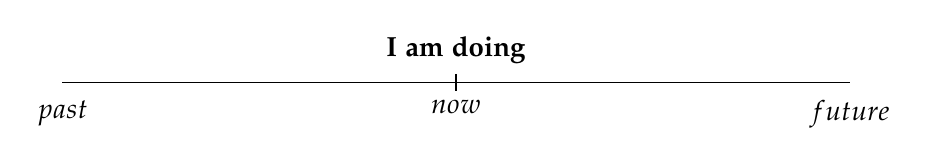
\begin{tikzpicture}[]
    % draw horizontal line
    \draw[] (0,0) -- (10,0);

    % draw vertical lines
    \foreach \x in {5}
    \draw (\x cm,3pt) -- (\x cm,-3pt);

    % draw nodes
    \draw (0,0) node[below=3pt] {$ past $} node[above=3pt] {$   $};
    \draw (5,0) node[below=3pt] {$ now $} node[above=3pt] {$ \textbf{I am doing} $};
    \draw (10,0) node[below=3pt] {$ future $} node[above=3pt] {$ $};
\end{tikzpicture}

\section{Present simple (I do)}
\label{Present imple}
$\textbf{drive(s), work(s), do(es)}$ etc. is the \textit{present simple}
\begin{flushleft}
\begin{tabular}{ | l l | }
 \hline
 I/we/you/they & $\textbf{drive/work/do}$ etc. \\
 \hline
 he/she/it & $\textbf{drives/works/does}$ etc. \\
 \hline
\end{tabular}
\end{flushleft}
We use the present simple to talk about things in general.\\
We use it to say that something happens all the time or repeatedly, or that something is true in general.\\
We use $\textbf{do/does}$ to make questions sentences
\begin{flushleft}
\newcommand{\tabincell}[2]{\begin{tabular}{@{}#1@{}}#2\end{tabular}}
\begin{tabular}{ | l | l | l | }
 \hline
 \tabincell{c}{\textbf{do}\\\textbf{does}} & \tabincell{l}{I/we/you/they\\he/she/it} & \tabincell{l}{\textbf{work}?\\\textbf{drive}?\\\textbf{do}?} \\ 
 \hline
\end{tabular}
\end{flushleft}
We use $\textbf{do/does}$ to make negative sentences
\begin{flushleft}
\newcommand{\tabincell}[2]{\begin{tabular}{@{}#1@{}}#2\end{tabular}}
\begin{tabular}{ | l | l | l | }
 \hline
 \tabincell{c}{I/we/you/they\\ he/she/it} & \tabincell{l}{\textbf{don't}\\ \textbf{doesn't}} & \tabincell{l}{\textbf{work}\\ \textbf{drive}\\ \textbf{do}} \\
 \hline
\end{tabular}
\end{flushleft}
In the following examples, $\textbf{do}$ is also the main verb (do you $\textbf{do}$ / doesn't $\textbf{do}$ etc.) \\
We use the present simple to say how often we do things. \\
We use the simple for things in general or things that happen repeatedly. \\
We use the simple for $\textit{permanent}$situations (things that continue for a long time). \\
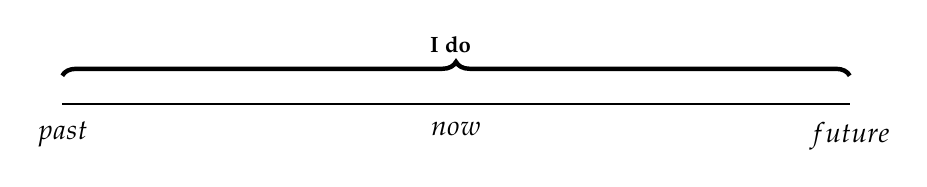
\begin{tikzpicture}[]
    % draw horizontal line
    \draw[] (0,0) -- (10,0);

    % draw nodes
    \draw (0,0) node[below=3pt] {$ past $} node[above=3pt] {$   $};
    \draw (5,0) node[below=3pt] {$ now $} node[above=3pt] {$ $};
    \draw (10,0) node[below=3pt] {$ future $} node[above=3pt] {$ $};
    \draw [black, ultra thick ,decorate,decoration={brace,amplitude=5pt}, yshift=-4pt] (0,0.5)  -- (10,0.5)  node [black,midway,above=4pt,xshift=-2pt] {\footnotesize $\textbf{I do}$};
\end{tikzpicture}

\section{Present perfect 1 (I have done)}
\label{Present perfect 1}
$\textbf{have lost / has lost}$ is the $\textit{present perfect simple}$ \\
The present perfect simple is $\textbf{have/has}$ + $\textbf{past participle}$. \\
\begin{flushleft}
\newcommand{\tabincell}[2]{\begin{tabular}{@{}#1@{}}#2\end{tabular}}
\begin{tabular}{ | l | l | l | }
 \hline
 \tabincell{c}{I/we/they/you\\ he/she/it} & \tabincell{l}{\textbf{have}\\ \textbf{has}} & \tabincell{l}{\textbf{finished}\\ \textbf{lost}\\ \textbf{done}\\ \textbf{been} etc.} \\
 \hline
\end{tabular}
\end{flushleft}
When we say `something $\textbf{has happened}$', this is usually new information.
When we use the present perfect, there is a connection with $\textit{now}$. The action in the past has a result $\textit{now}$
Compare $\textbf{gone (to)}$ and $\textbf{been (to)}$
\begin{itemize}
    \item[$\square$] He $\textbf{has gone to}$ (= he is there now or on his way there)
    \item[$\square$] She $\textbf{has been}$ (= she has now come back)
\end{itemize}
$\textbf{Just}$ = a short time ago \\
$\textbf{Already}$ = sooner than expected \\
$\textbf{Yet}$ = until now. We use $\textbf{yet}$ to show that we are expecting something to happen. \\

\section{Present perfect 2 (I have done)}
\label{Present perfect 2}
When we talk about a period of time that continues from the past until now, we use the $\textit{present perfect}$ ($\textbf{have been / have travelled}$ etc.).
$\textbf{been (to)}$ = visited
In the following examples too, the speakers are talking about a period that continues until now ($\textbf{recently, in the last few days, so far, since I arrived}$ etc.) \\
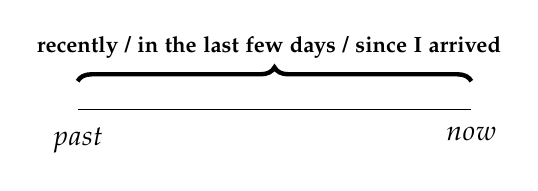
\begin{tikzpicture}[]
    % draw horizontal line
    \draw[] (0,0) -- (5,0);

    % draw nodes
    \draw (0,0) node[below=3pt] {$ past $} node[above=3pt] {$   $};
    \draw (5,0) node[below=3pt] {$ now $} node[above=3pt] {$ $};
    \draw [black, ultra thick ,decorate,decoration={brace,amplitude=5pt}, yshift=-4pt] (0,0.5)  -- (5,0.5)  node [black,midway,above=4pt,xshift=-2pt] {\footnotesize $\textbf{recently / in the last few days / since I arrived}$};
\end{tikzpicture} \\
In the same way we use the present perfect with $\textbf{today, this evening, this year}$ etc. when these periods are not finished at the time of speaking. \\
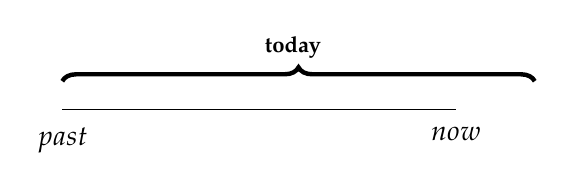
\begin{tikzpicture}[]
    % draw horizontal line
    \draw[] (0,0) -- (5,0);

    % draw nodes
    \draw (0,0) node[below=3pt] {$ past $} node[above=3pt] {$   $};
    \draw (5,0) node[below=3pt] {$ now $} node[above=3pt] {$ $};
    \draw [black, ultra thick ,decorate,decoration={brace,amplitude=5pt}, yshift=-4pt] (0,0.5)  -- (6,0.5)  node [black,midway,above=4pt,xshift=-2pt] {\footnotesize $\textbf{today}$};
\end{tikzpicture} \\
We say `It's the (first) time something $\textbf{has happened}$'. For example:
\begin{itemize}
    \item[$\square$] It's the first time he $\textbf{has driven}$ a car. (not drives)
    \item[$\square$] He $\textbf{hasn't driven}$ a car $\textbf{before}$.
    \item[$\square$] He $\textbf{has never driven}$ a car $\textbf{before}$.
\end{itemize}
In the same way we say:
\begin{itemize}
    \item[$\square$] Sarah has lost her passport again. This is the second time this $\textbf{has happened}$. ($\textit{not}$ happens)
    \item[$\square$] Andy is phoning his girlfriend again. It's the third time he$\textbf{'s phoned}$ her $\textbf{this evening}$.
\end{itemize}

\section{Present perfect continuous (I have been doing)}
\label{Present perfect continuous}
$\textbf{have/has been}$ + $\textbf{-ing}$ is the $\textit{present perfect continuous}$
\begin{flushleft}
\newcommand{\tabincell}[2]{\begin{tabular}{@{}#1@{}}#2\end{tabular}}
\begin{tabular}{ | l | l | l | l | }
 \hline
 \tabincell{c}{I/we/they/you\\ he/she/it} & \tabincell{l}{\textbf{have}\\ \textbf{has}} & \tabincell{l}{\textbf{been}} & \tabincell{l}{\textbf{doing}\\ \textbf{working}\\ \textbf{learning} etc.} \\
 \hline
\end{tabular}
\end{flushleft}
We use the present perfect continuous for an activity that has recently stopped or just stopped. \\
You can use the present perfect continuous for repeated actions.

\section{Present tenses (I am doing / I do) for the future}
\label{Present tenses (I am doing / I do) for the future}
$\textbf{I'm doing}$ something (tomorrow etc.) = I have already decided and arranged to do it. \\
We do not normally use $\textbf{will}$ to talk about what we have arranged to do. \\
We also use the present continuous for an action $\textit{just before you start to do it}$. This happens especially with verbs of movement($\textbf{go/come/leave}$ etc.). For example:
\begin{itemize}
    \item[$\square$] I'm tired. I$\textbf{'m going}$ tobed now. Goodnight. ($\textit{not}$ I go to bed now)
    \item[$\square$] `Tina, are you ready yet?' `Yes, I$\textbf{'m coming.}$' ($\textit{not}$ I come)
\end{itemize}
We use the present simple when we talk about timetables and programmes (for example, transport or cinema times). \\
You can use the present simple to talk about people if their plans are fixed like a timetable. \\
But the continuous is more usual for other personal arrangements. \\
Compare: \\
Present continuous
\begin{itemize}
    \item[$\square$] What time $\textbf{are}$ you $\textbf{arriving}$?
    \item[$\square$] I$\textbf{'m going}$ to the cinema this evening.
\end{itemize}
Present simple
\begin{itemize}
    \item[$\square$] What time $\textbf{does}$ the train $\textbf{arrive}$?
    \item[$\square$] The film $\textbf{starts}$ at 8.15.
\end{itemize}
When you talk about appointments, lessons, exams etc., you can use $\textbf{I have}$ or $\textbf{I've got}$
\begin{itemize}
    \item[$\square$] $\textbf{I have}$ an exam next week.\qquad or \qquad$\textbf{I've got}$ an exam next week.
\end{itemize}


\chapter{Past}\label{ch:2}
\section{Past simple (I did)}
\label{Past simple (I did)}
\textbf{lived/started/wrote/was/died} are all \textit{past simple}
In questions and negative sentences we use \textbf{did/didn't} + infinitive (\textbf{enjoy/see/go} etc.)
\begin{flushleft}
\newcommand{\tabincell}[2]{\begin{tabular}{@{}#1@{}}#2\end{tabular}}
\begin{tabular}{ | l | l | }
 \hline
 \tabincell{c}{I\\ she\\ they} & \tabincell{l}{enjoy\textbf{ed}\\ \textbf{saw}\\ \textbf{went}} \\
 \hline
\end{tabular}
\end{flushleft}
\begin{flushleft}
\newcommand{\tabincell}[2]{\begin{tabular}{@{}#1@{}}#2\end{tabular}}
\begin{tabular}{ | l | l | l | }
 \hline
 \tabincell{l}{\textbf{did}} & \tabincell{c}{you\\ she\\ they} & \tabincell{l}{\textbf{enjoy}?\\ \textbf{see}?\\ \textbf{go}?} \\
 \hline
\end{tabular}
\end{flushleft}
\begin{flushleft}
\newcommand{\tabincell}[2]{\begin{tabular}{@{}#1@{}}#2\end{tabular}}
\begin{tabular}{ | l | l | l | }
 \hline
 \tabincell{c}{I\\ she\\ they} & \tabincell{l}{\textbf{didn't}} & \tabincell{l}{\textbf{enjoy}\\ \textbf{see}\\ \textbf{go}} \\
 \hline
\end{tabular}
\end{flushleft}
Sometimes \textbf{do} is the main verb in the sentence (did you \textbf{do}?, I didn't \textbf{do})
\begin{itemize}
    \item[$\square$] What \textbf{did} you \textbf{do} at the weekend? (\textit{not} What did you at the weekend?)
    \item[$\square$] I \textbf{didn't do} anything. (\textit{not} I didn't anything)
\end{itemize}
The past of \textbf{be} (\textbf{am/is/are}) is \textbf{was/were}
\begin{flushleft}
\begin{tabular}{ | l l | }
 \hline
 I/he/she/it      & \textbf{was/wasn't} \\
 \hline
 we/you/they      & \textbf{were/weren't} \\
 \hline
\end{tabular}
\end{flushleft}
In questions sentences
\begin{flushleft}
\begin{tabular}{ | l l | }
 \hline
 \textbf{was}       & I/he/she/it? \\
 \hline
 \textbf{were}      & we/you/they? \\
 \hline
\end{tabular}
\end{flushleft}

\section{Past continuous (I was doing)}
\label{Past continuous (I was doing)}
\textbf{was/were + -ing} is the past continuous
\begin{flushleft}
\newcommand{\tabincell}[2]{\begin{tabular}{@{}#1@{}}#2\end{tabular}}
\begin{tabular}{ | l | l | l | }
 \hline
 \tabincell{c}{he/she/it\\ we/you/they} & \tabincell{l}{\textbf{was}\\ \textbf{were}} & \tabincell{l}{\textbf{playing}\\ \textbf{doing}\\ \textbf{working} etc.} \\
 \hline
\end{tabular}
\end{flushleft}
I \textbf{was doing} something = I was in the middle of doing it at a certain time. The action or situation started before this time, but had not finished. \\
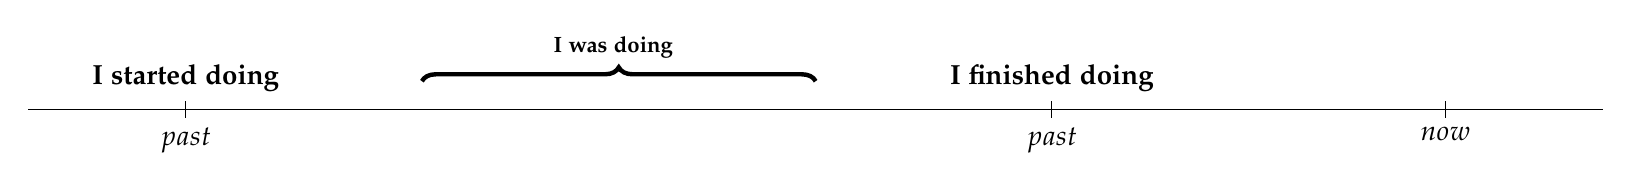
\begin{tikzpicture}[]
    % draw horizontal line
    \draw[] (0,0) -- (20,0);

    % draw vertical lines
    \foreach \x in {2,13,18}
    \draw (\x cm,3pt) -- (\x cm,-3pt);

    % draw nodes
    \draw (2,0) node[below=3pt] {$ past $} node[above=3pt] {$ \textbf{I started doing} $};
    \draw (13,0) node[below=3pt] {$ past $} node[above=3pt] {$ \textbf{I finished doing} $};
    \draw (18,0) node[below=3pt] {$ now $} node[above=3pt] {$ $};
    \draw [black, ultra thick ,decorate,decoration={brace,amplitude=5pt}, yshift=-4pt] (5,0.5)  -- (10,0.5)  node [black,midway,above=4pt,xshift=-2pt] {\footnotesize $\textbf{I was doing}$};
\end{tikzpicture}
Compare I \textbf{was doing} (\textit{past continuous}) and I \textbf{did} (\textit{past simple}) \\
I \textbf{was doing} (= in the middle of an action)
\begin{itemize}
    \item[$\square$] We were \textbf{walking} home when I met Dan. (in the middle of walking home)
    \item[$\square$] Kate \textbf{was watching} TV when we arrived.
\end{itemize}
I \textbf{did} (= complete action)
\begin{itemize}
    \item[$\square$] We \textbf{walked} home after the party last night. (= all the way, completely)
    \item[$\square$] Kate \textbf{watched} TV a lot when she was ill last year.
\end{itemize}
You can say that something \textbf{happened} (past simple) in the middle of something else (past continuous). \\
But we use the past simple to say that one thing happened \textit{after} another. \\
Compare
\begin{itemize}
    \item[$\square$] When Karen arrived, we \textbf{were having} dinner. (= we had already started before she arrived)
    \item[$\square$] When Karen arrived, we \textbf{had} dinner. (= Karen arrived, and then we had dinner)
\end{itemize}

\section{Past perfect (I had done)}
\label{Past perfect (I had done)}
\textbf{had gone} is the \textit{past perfect}
\begin{flushleft}
\newcommand{\tabincell}[2]{\begin{tabular}{@{}#1@{}}#2\end{tabular}}
\begin{tabular}{ | l | l | l | }
 \hline
 \tabincell{c}{I/we/they/you\\ he/she/it} & \tabincell{l}{\textbf{had}} & \tabincell{l}{\textbf{gone}\\ \textbf{seen}\\ \textbf{finished} etc.} \\
 \hline
\end{tabular}
\end{flushleft}
The past perfect (simple) is \textbf{had} + \textit{past participle} (\textbf{gone/seen/finished} etc.). \\
Sometimes we talk about something that happened in the past. \\
Compare \textit{present perfect} (\textbf{have seen} etc.) and \textit{past perfect} (\textbf{had seen} etc.) \\
Present perfect \\
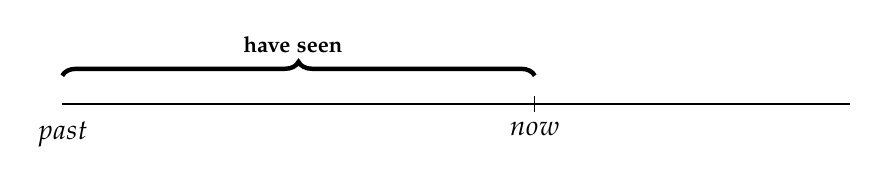
\begin{tikzpicture}[]
    % draw horizontal line
    \draw[] (0,0) -- (10,0);

    % draw vertical lines
    \foreach \x in {6}
    \draw (\x cm,3pt) -- (\x cm,-3pt);

    % draw nodes
    \draw (0,0) node[below=3pt] {$ past $} node[above=3pt] {$ $};
    \draw (6,0) node[below=3pt] {$ now $} node[above=3pt] {$ $};
    \draw [black, ultra thick ,decorate,decoration={brace,amplitude=5pt}, yshift=-4pt] (0,0.5)  -- (6,0.5)  node [black,midway,above=4pt,xshift=-2pt] {\footnotesize $\textbf{have seen}$};
\end{tikzpicture} \\
Past perfect \\
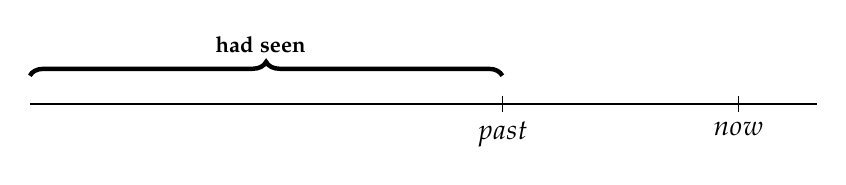
\begin{tikzpicture}[]
    % draw horizontal line
    \draw[] (0,0) -- (10,0);

    % draw vertical lines
    \foreach \x in {6, 9}
    \draw (\x cm,3pt) -- (\x cm,-3pt);

    % draw nodes
    \draw (6,0) node[below=3pt] {$ past $} node[above=3pt] {$ $};
    \draw (9,0) node[below=3pt] {$ now $} node[above=3pt] {$ $};
    \draw [black, ultra thick ,decorate,decoration={brace,amplitude=5pt}, yshift=-4pt] (0,0.5)  -- (6,0.5)  node [black,midway,above=4pt,xshift=-2pt] {\footnotesize $\textbf{had seen}$};
\end{tikzpicture} \\
Compare \textit{past simple} (\textbf{left}, \textbf{was} etc.) and \textit{past perfect} (\textbf{had left}, \textbf{had been} etc.)

\section{Past perfect continuous (I had been doing)}
\label{Past perfect continuous (I had been doing)}
\textbf{had been -ing} is the \textit{past perfect continuous}
\begin{flushleft}
\newcommand{\tabincell}[2]{\begin{tabular}{@{}#1@{}}#2\end{tabular}}
\begin{tabular}{ | l | l | l | l | }
 \hline
 \tabincell{c}{I/we/they/you\\ he/she/it} & \tabincell{l}{\textbf{had}} & \tabincell{l}{\textbf{been}}  & \tabincell{l}{do\textbf{ing}\\ work\textbf{ing}\\ play\textbf{ing} etc.} \\
 \hline
\end{tabular}
\end{flushleft}
You can say that something \textbf{had been happening} before something else happened.
\begin{itemize}
    \item[$\square$] We\textbf{'d been playing} tennis for about half an hour when it \textbf{started} to rain heavily.
\end{itemize}
Compare \textbf{have been -ing} (\textit{present perfect continuous}) and \textbf{had been -ing} (\textit{past perfect continuous}).
Present perfect continuous \\
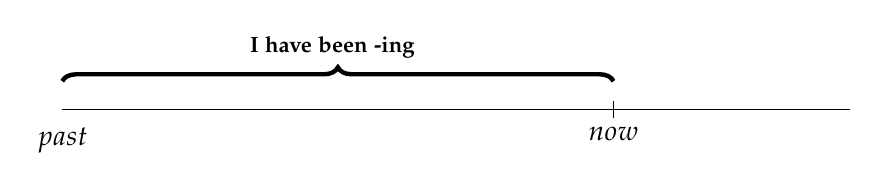
\begin{tikzpicture}[]
    % draw horizontal line
    \draw[] (0,0) -- (10,0);

    % draw vertical lines
    \foreach \x in {7}
    \draw (\x cm,3pt) -- (\x cm,-3pt);

    % draw nodes
    \draw (0,0) node[below=3pt] {$ past $} node[above=3pt] {$ $};
    \draw (7,0) node[below=3pt] {$ now $} node[above=3pt] {$ $};
    \draw [black, ultra thick ,decorate,decoration={brace,amplitude=5pt}, yshift=-4pt] (0,0.5)  -- (7,0.5)  node [black,midway,above=4pt,xshift=-2pt] {\footnotesize $\textbf{I have been -ing}$};
\end{tikzpicture} \\
Past perfect continuous \\
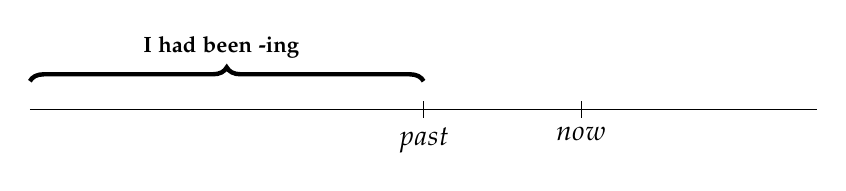
\begin{tikzpicture}[]
    % draw horizontal line
    \draw[] (0,0) -- (10,0);

    % draw vertical lines
    \foreach \x in {5,7}
    \draw (\x cm,3pt) -- (\x cm,-3pt);

    % draw nodes
    \draw (5,0) node[below=3pt] {$ past $} node[above=3pt] {$ $};
    \draw (7,0) node[below=3pt] {$ now $} node[above=3pt] {$ $};
    \draw [black, ultra thick ,decorate,decoration={brace,amplitude=5pt}, yshift=-4pt] (0,0.5)  -- (5,0.5)  node [black,midway,above=4pt,xshift=-2pt] {\footnotesize $\textbf{I had been -ing}$};
\end{tikzpicture} \\
Compare \textbf{was -ing} (\textit{past continuous}) and \textbf{had been -ing}
\begin{itemize}
    \item[$\square$] It \textbf{wasn't raining} when we went out. The sun \textbf{was shining}. But it \textbf{had been raining}, so the ground was wet.
    \item[$\square$] Katherine \textbf{was lying} on the sofa. She was tired because she\textbf{'d been working} hard.
\end{itemize}


%\chapter{Citations and Links}\label{ch:3}
%\section{Introduction}
Some people just cite papers in introductions for no reason.

\section{Setup}
\label{sec:potent-outc-fram}
\blindmathtrue\blindtext\ See Figure \ref{fig:figure1} for illustration.
\begin{figure}[ht]
  \centering
\begin{verbatim}
#include <iostream>
int main(int argc, char** argv) {
  std::cout << "Hello World." << std::endl;
  return 0;
}
\end{verbatim}
  \caption{Captions for figures go at the bottom of the figure.}
  \label{fig:figure1}
\end{figure}

\section{Conclusion}
\blindmathfalse\blindtext[2]


%\chapter{Other Formats}\label{ch:4}
%\section{Introduction}
Some people just cite papers in introductions for no reason.

\section{Setup}
\label{sec:potent-outc-fram}
\blindmathtrue\blindtext\ See Figure \ref{fig:figure1} for illustration.
\begin{figure}[ht]
  \centering
\begin{verbatim}
#include <iostream>
int main(int argc, char** argv) {
  std::cout << "Hello World." << std::endl;
  return 0;
}
\end{verbatim}
  \caption{Captions for figures go at the bottom of the figure.}
  \label{fig:figure1}
\end{figure}

\section{Conclusion}
\blindmathfalse\blindtext[2]


% Put appendices, bibliography, and supplemental materials here

% The bibliography may be single spaced within each entry, but must be
% double-spaced between each entry. Most bibliography styles leave space between
% entries, so that shouldn't be a problem.
%\begin{singlespacing}
  % I like "References" better than "Bibliography"
%  \renewcommand{\bibname}{References}

  % Any bibliohgraphy style that leaves space between entries is fine
%  \nocite{*}
%  \bibliographystyle{acm}
%  \bibliography{references/references}
%\end{singlespacing}

% Appendices from all chapters should go at the end
%\begin{appendices}

\chapter{Appendix to Chapter \ref{ch:1}}\label{cha:append-chapt-refch:1}

\section{Auxiliary Lemmata}
Fundamental identity
\begin{equation}
  \label{eq:A}
  e^{i\pi}=-1.
\end{equation}
Equivalence relation
\begin{equation}
  \label{eq:B}
  A=B.
\end{equation}

\section{Proofs}

\chapter{Appendix to Chapter \ref{ch:3}}

\section{Proofs}

\section{Supplementary Tables and Figures}
\begin{longtable}{cc}
% Caption to appear on the first page and in the list of tables
\caption[Optional Short caption (used in list of tables)]{A long table} \label{grid_mlmmh} \\

Heading that appears & on first page only\\
\hline
\endfirsthead
\caption[]{(continued)}\\
Heading that appears & on all pages\\
\hline
\endhead
% optional footer
\hline \multicolumn{2}{r}{{Continued on next page}} \\
\endfoot
% footer to appear on tha last page (empty)
\endlastfoot

Contrary to popular & belief, Lorem Ipsum \\ is & not \\ simply &
random \\ text &. It \\ has & roots \\ in & a \\ piece & of \\ classical & Latin
\\ literature & from \\ 45 & BC \\, making & it \\ over & 2000 \\ years old. Richard & Mc \\Clintock &, a \\ Latin & professor \\ at & Hampden \\-Sydney
& College \\ in & Virginia \\, looked & up \\ one & of \\ the & more
\\obscure & Latin \\ words &, consectetur \\, from & a \\ Lorem & Ipsum \\
passage &, and \\ going & through \\ the & cites \\ of & the word in \\
classical & literature , discovered the \\ undoubtable & source. Lorem Ipsum
\\ comes & from \\ sections & 1 \\.10 &.32 \\ and & 1 \\.10 &.33 \\ of
&"de \\ Finibus & Bonorum \\ et & Malorum \\" (The & Extremes \\ of & Good \\
and & Evil \\) by & Cicero \\, written & in \\ 45 & BC \\. This & book \\ is & a
\\ treatise & on \\ the & theory \\ of & ethics \\, very & popular \\ during
&the \\ Renaissance &. The \\ first & line \\ of & Lorem \\ Ipsum, "Lorem ipsum
& dolor \\ sit & amet \\..", comes from a & line \\ in & section
1.10.32.\\
\end{longtable}


\begin{sidewaysfigure}
  \centering Supplementary figures and tables should be placed in the appendix,
  not at the end of a chapter. To rotate big tables and figures $90^{\circ}$,
  use the rotating package and the sidewaystable and sidewaysfigure
  environments. This ensures that the figure and caption get rotated, but the
  page number stays at the bottom of the page.
  \caption{Supplementary Figure}
  \label{fig:figuresup1}
\end{sidewaysfigure}

\begin{figure}[ht]
  \centering
  This is another supplementary figure.
  \caption{Another Figure}
  \label{fig:figuresup3}
\end{figure}


\end{appendices}


\end{document}
